\documentclass[11pt, oneside]{article}   	% use "amsart" instead of "article" for AMSLaTeX format
\usepackage{geometry}                		% See geometry.pdf to learn the layout options. There are lots.
\geometry{letterpaper}                   		% ... or a4paper or a5paper or ... 
%\geometry{landscape}                		% Activate for for rotated page geometry
%\usepackage[parfill]{parskip}    		% Activate to begin paragraphs with an empty line rather than an indent
\usepackage{graphicx}				% Use pdf, png, jpg, or eps§ with pdflatex; use eps in DVI mode
								% TeX will automatically convert eps --> pdf in pdflatex		
\usepackage{amssymb}
\usepackage{minted}
\usepackage{hyperref}
%\usemintedstyle{bw}

\graphicspath{{figures/}}

\usepackage{lmodern}% http://ctan.org/pkg/lm
\setlength\parindent{0pt}

\title{Literature Repo User Guide}
\author{Gunnar}
%\date{}							% Activate to display a given date or no date

\begin{document}

\maketitle

This guide explains how to use the group's literature repository together with BibDesk. BibDesk is a free mac program that is a front end for a bibtex .bib file.  It allows GUI-based manipulation of the database, easy importation of new references, and most importantly linking to a PDF of the article itself.

\section{ssh key}
First you need to create an ssh key that will identify you on the server. That way you don't have to type a password every time you want to sync your repo with the server. Open up a terminal and go to your home directory
\begin{minted}[numbersep=5pt]{sh}
cd ~
\end{minted}
See if you have an ssh directory already:
\begin{minted}[numbersep=5pt]{sh}
ls .ssh
\end{minted}
If you don't have the directory yet (you will see something like ls: .ssh: No such file or directory) then create it:
\begin{minted}[numbersep=5pt]{sh}
mkdir .ssh
chmod 700 .ssh
\end{minted}
Now change into the ssh directory and look around you:
\begin{minted}[numbersep=5pt]{sh}
cd .ssh
ls
\end{minted}
If you happen to see two files names id\_rsa and id\_rsa.pub then skip the following skip. Otherwise create a key:
\begin{minted}[numbersep=5pt]{sh}
ssh-keygen -f id_rsa -t rsa -q
\end{minted}
Now add the key to the ssh agent:
\begin{minted}[numbersep=5pt]{sh}
ssh-add id_rsa
\end{minted}
The next step is to email me (gvoet@ucsd.edu) the contents of id\_rsa.pub. You could for example type
\begin{minted}[numbersep=5pt]{sh}
less id_rsa.pub
\end{minted}
and then copy and paste the output to an email. I will copy your public key to the server.

\section{git}
If you are working on a Mac your system should come with git pre-installed. Now set your name and email address, this will later identify you when you push your changes to the server. Run the two following commands after you modify them:
\begin{minted}[numbersep=5pt]{sh}
git config --global user.name "Your Name"
git config --global user.email email@example.com
\end{minted}
This should have created a file named .gitconfig in your home directory. Open .gitconfig with your editor of choice and add the following settings as new lines after your name and email:
\begin{minted}[]{sh}
[push]
  default = simple
[alias]
  ca = !sh -c 'git add -A && git commit -m \"$1\" && git push' -
[core]
  precomposeunicode = false
\end{minted}

Now go to the directory where you want the literature repo to reside. It will come within it's own folder, so no need to create one extra directory level. This means if you go to your home directory now, the repo will be at /Users/yourhome/wavebib/. Choose any place you like! Now you are ready to clone the repository. This may take a while as it will copy a ton of pdfs that are already in there. Note that your ssh key has to be on the server for this to work!
\begin{minted}[numbersep=5pt]{sh}
git clone gituser@kipapa.ucsd.edu:/Users/gituser/repo/wavebib/
\end{minted}



%
%In the users home directory, create an ssh key if not existent yet:
%mkdir .ssh (if it doesn't exist)
%chmod 700 .ssh
%cd .ssh
%ssh-keygen -f id_rsa -t rsa -q
%ssh-add id_rsa
%
%EMAIL SSH KEY
%email public key to Gunnar, he will add it to the server
%
%GIT
%Set your user name and email address
%git config --global user.name "John Doe"
%git config --global user.email johndoe@example.com
%
%Go to where you want the repo directory to reside. It will come within it's own folder, so no need to create one extra directory level.
%git clone gituser@kipapa.ucsd.edu:/Users/gituser/repo/wavebib/
%
%GIT ALIAS
%Add this to ~/.gitconfig
%[alias]
%  ca = !sh -c 'git add -A && git commit -m \"$1\" && git push' -
%
%git ca "your comment"
%
%also add this to ~/.gitfonfig? Not sure if this is really needed/helpful...
%[core]
%  precomposeunicode = false
%
%TO PULL CHANGES FROM THE SERVER
%git pull
%
%TO APPLY LOCAL CHANGES TO THE SERVER
%git ca "short comment of what you did"
%or
%git add file1 file2
%git commit -m "short comment of what you did"
%git push
%or
%git add -A
%git commit -m "short comment of what you did"
%git push
%
%INFO
%git log --stat


\section{BibDesk}
Once the repository has downloaded you can start right away.  To get set up, open the main.bib file in BibDesk.  You'll be able to browse all the articles in the main.bib database (thousands of articles).  Many are linked to a PDF, which you should just be able to click on. To use the database most effectively and easily, make three changes in BibDesk preferences:
\begin{enumerate}
\item In 'General', set BibDesk to open the main.bib file upon starting. 
\item Under 'Autofile' select 'File papers relative to each document' and check 'File papers automatically'. For 'local file format' select Custom and enter the following string (by clicking 'advanced'): \mint{sh}|articles/%a1/%a1%Y%u0.pdf|
Fig.~\ref{fig:autofile} summarizes the settings in 'Autofile'.
\item Unfortunately, BibDesk can't generate the cite keys the way we want them, so under 'Cite Key Format' leave 'Autogenerate' unchecked.
\end{enumerate}

Now, you can easily import new articles by simply dragging the PDF onto the reference in BibDesk. BibDesk will automatically file the paper. The format string tells it to store the articles in a folder by the author's last name, and to name them as (e.g.) Zhang2012a.pdf.  If you add new references, please follow the convention we use for the cite key; e.g. zhangetal12, alfordgregg01a, etc.


\begin{figure}[h]
   \centering
   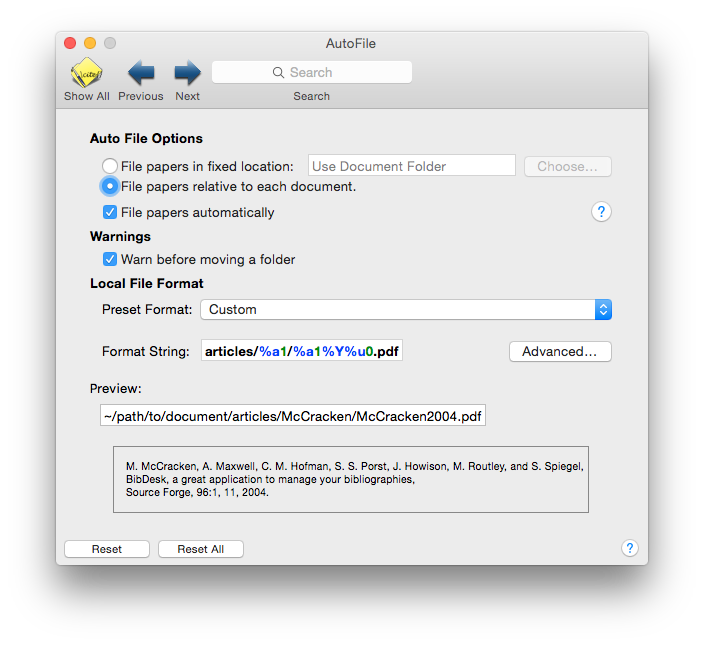
\includegraphics[width=1.0\textwidth]{bibdesk_autofile.png} % requires the graphicx package
   \caption{BibDesk AutoFile settings}
   \label{fig:autofile}
\end{figure}


\section{TexShop}

Using BibDesk is really easy in TexShop. Make sure to check 'BibDeskCompletions' in the main preference pane. Once you have AutoCompletion setup, you can simply type part of the cite key in TexShop and hit Esc, and it will fill in the key from the database for you, letting you choose from a pulldown menu if there are multiples.

\section{Making Changes}

If this is going to be useful, we ALL have to have good practices for updating our changes. You 'check in' and 'check out' versions from the repository with the commands below. If you run into trouble, contact me (Gunnar) and we'll figure out how to merge different versions or how to get rid of unwanted changes.  
	Here are the steps. 
	
\begin{enumerate}
\item Before making any changes, make sure you are current by first closing main.bib or quitting BibDesk, and (from the terminal window on your computer from the directory in which you have stored the database) typing
\mint{sh}|git pull|
This will make sure you have the latest version from the server.

\item Make your changes in the .bib file, add pdfs... Make sure you save the .bib file when you are done! You can then review your changes by typing
\mint{sh}|git status|

\item Now you push your changes to the server using the alias you created earlier in your .gitconfig-file:
\mint{sh}|git ca "your short comment"|
Please provide something meaningful in the comment, like the cite key of the entry you just added. Don't worry about it too much though if you just added a lot. Also, your name gets written to the log automatically, so no need to add your name to the comment. If everything is running smoothly your updates should now be up on the server and available to all other users.

\end{enumerate}

Note that the alias 'git ca' is just a short form of the more general git workflow for adding changes and new files to the repository. You could also add your changes with the following commands that 1) add all changes 2) commit them and 3) push them to the server:
\begin{minted}[numbersep=5pt]{sh}
git add -A
git commit -m "your comment"
git push
\end{minted}

\section{Tips \& Tricks}
\begin{itemize}
\item On google scholar, if you go to Scholar preferences/Bibliography manager, you can select "Show links to import citations into Bibtex."  Then you can just copy the citation info and paste it from the clipboard into BibDesk.

\item To look up journal abbreviations (it's nice to have them consistent) go to\\
 \href{http://woodward.library.ubc.ca/research-help/journal-abbreviations/}{http://woodward.library.ubc.ca/research-help/journal-abbreviations/}

\item You can link main.bib to your local texmf settings, that way you can include the file with the simple command
\mint{latex}|\bibliography{main}|
in any latex file. To link the file, type
\mint{bash}|ln -s /your/path/to/your/main.bib ~/Library/texmf/bibtex/bib/main.bib|
\end{itemize}

\begin{figure}[h]
   \centering
   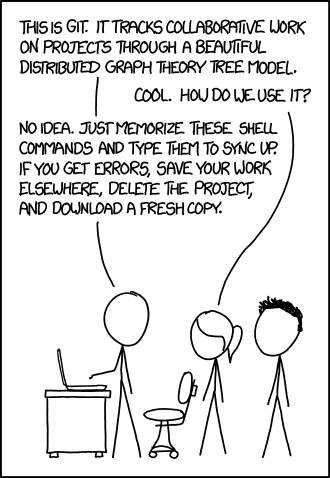
\includegraphics[width=1.0\textwidth]{git.png} % requires the graphicx package
%   \caption{BibDesk }
   \label{fig:git}
\end{figure}

\end{document}  